% IEEEAerospace2012.cls requires the following packages: times, rawfonts, oldfont, geometry
\documentclass[twocolumn,letterpaper]{IEEEAerospaceCLS}  % only supports two-column, letterpaper format

% The next line gives some packages you may find useful for your paper--these are not required though.
%\usepackage[]{graphicx,float,latexsym,amssymb,amsfonts,amsmath,amstext,times,psfig}
% NOTE: The .cls file is now compatible with amsmath!!!

\usepackage{amsmath,amssymb,url}
\usepackage{graphicx,subfigure,tikz}
\usepackage{color}
\usepackage{wrapfig}
\usepackage{epstopdf}
\newcommand{\ignore}[1]{}  % {} empty inside = %% comment

\newcommand{\norm}[1]{\ensuremath{\left\| #1 \right\|}}
\newcommand{\bracket}[1]{\ensuremath{\left[ #1 \right]}}
\newcommand{\braces}[1]{\ensuremath{\left\{ #1 \right\}}}
\newcommand{\parenth}[1]{\ensuremath{\left( #1 \right)}}
\newcommand{\pair}[1]{\ensuremath{\langle #1 \rangle}}
\newcommand{\met}[1]{\ensuremath{\langle\langle #1 \rangle\rangle}}
\newcommand{\refeqn}[1]{(\ref{eqn:#1})}
\newcommand{\reffig}[1]{Fig. \ref{fig:#1}}
\newcommand{\tr}[1]{\mathrm{tr}\ensuremath{\negthickspace\bracket{#1}}}
\newcommand{\trs}[1]{\mathrm{tr}\ensuremath{[#1]}}
\newcommand{\ave}[1]{\mathrm{E}\ensuremath{[#1]}}
\newcommand{\deriv}[2]{\ensuremath{\frac{\partial #1}{\partial #2}}}
\newcommand{\SO}{\ensuremath{\mathsf{SO(3)}}}
\newcommand{\T}{\ensuremath{\mathsf{T}}}
\renewcommand{\L}{\ensuremath{\mathsf{L}}}
\newcommand{\so}{\ensuremath{\mathfrak{so}(3)}}
\newcommand{\SE}{\ensuremath{\mathsf{SE(3)}}}
\newcommand{\se}{\ensuremath{\mathfrak{se}(3)}}
\renewcommand{\Re}{\mathbb{R}}
\newcommand{\aSE}[2]{\ensuremath{\begin{bmatrix}#1&#2\\0&1\end{bmatrix}}}
\newcommand{\ase}[2]{\ensuremath{\begin{bmatrix}#1&#2\\0&0\end{bmatrix}}}
\newcommand{\D}{\ensuremath{\mathbf{D}}}
\renewcommand{\d}{\ensuremath{\mathfrak{d}}}
\newcommand{\Sph}{\ensuremath{\mathsf{S}}}
\renewcommand{\S}{\Sph}
\newcommand{\J}{\ensuremath{\mathbf{J}}}
\newcommand{\Ad}{\ensuremath{\mathrm{Ad}}}
\newcommand{\intp}{\ensuremath{\mathbf{i}}}
\newcommand{\extd}{\ensuremath{\mathbf{d}}}
\newcommand{\hor}{\ensuremath{\mathrm{hor}}}
\newcommand{\ver}{\ensuremath{\mathrm{ver}}}
\newcommand{\dyn}{\ensuremath{\mathrm{dyn}}}
\newcommand{\geo}{\ensuremath{\mathrm{geo}}}
\newcommand{\Q}{\ensuremath{\mathsf{Q}}}
\newcommand{\G}{\ensuremath{\mathsf{G}}}
\newcommand{\g}{\ensuremath{\mathfrak{g}}}
\newcommand{\Hess}{\ensuremath{\mathrm{Hess}}}
\newcommand\circled[1]{%
  \tikz[baseline=(C.base)]\node[draw,circle,inner sep=0.5pt](C) {#1};\!
}

\newtheorem{prop}{Proposition}


\newcommand{\EditTL}[1]{{\color{blue}\protect #1}}
%\newcommand{\EditTL}[1]{{\protect #1}}


\begin{document}
\title{Design and Development of a Free-Floating\\ Hexrotor UAV for 6-DOF Maneuvers}

\author{%
Evan Kaufman, Kiren Caldwell, Daewon Lee and Taeyoung Lee\\ 
Mechanical and Aerospace Engineering\\
George Washington University\\
Washington, DC 20052\\
202-994-8710\\
\{evankaufman, kiranimo, daewonlee, tylee\}@gwu.edu
%\and 
%Jane Smith\\
%Department of ECE\\
%University of Nowhere\\
%Nowhere, ZS 99999\\
%888-888-8888\\
%jane.smith@nowhere.edu
%%%% IMPORTANT: Use the correct copyright information--IEEE, Crown, or U.S. government. %%%%%
%\thanks{\footnotesize 978-1-4799-1622-1/14/$\$31.00$ \copyright2014 IEEE.}              % This creates the copyright info that is the correct 2012 data
%\thanks{{978-1-4799-1622-1/14/$\$31.00$ \copyright2014 Crown.}}          % Use this copyright notice only if you are employed by a crown government (e.g., Canada, UK, Australia)
%\thanks{{U.S. Government work not protected by U.S. copyright.}}         % Use this copyright notice only if you are employed by the U.S. Government.
%%%%% Use this footnote to keep track of your paper number/versioning.
\thanks{{\bf 978-1-4799-1622-1/14/\$31.00 \copyright2014 IEEE}} % NOTE: Modify this line to reflect your paper number, version, and date of version for tracking purposes.
}


\maketitle

\thispagestyle{plain}
\pagestyle{plain}

\begin{abstract}
This paper presents design and development of an experimental testbed for nonlinear geometric controls of a rigid body. We develop a fully actuated hexrotor UAV that uses six variable pitch propellers to control six degrees of freedom maneuvers, namely three position and three attitude variables, independently. In contrast to the popular quadrotor UAVs that can hover at a single attitude, the hexrotor presented in this paper is capable of hovering at any attitude provided that thrust is sufficiently large. A geometric controller is also developed on the special Euclidean group to track given desired position and attitude trajectories under the effects of unknown disturbances. These are particularly useful for ground tests for large angle rotational dynamics of spacecraft that are combined with arbitrary translational motions. A numerical example that involves a nontrivial maneuver and preliminary experimental tests are also presented.
%
%
%It is well known that a controller that considers the geometric properties of the special euclidean group  explicitly may be applied to a fully-actuated system; this paper provides a technique to validate this controller, particularly to model rotations in spacecraft maneuvers.  We present a numerical example that involves a nontrivial trajectory and preliminary experimental results.
\end{abstract}


\tableofcontents

\section{Introduction}

Quadrotor UAVs have become popular recently due to their simple mechanical structure and aggressive maneuverability. However, a quadrotor can only hover at a single attitude where the plane of its rotors is orthogonal to gravity. This restriction causes the attitude dynamics to be coupled with the translational dynamics, yielding a platform not conducive to spacecraft attitude control problems that involve arbitrary rotational maneuvers or de-tumbling. Other spacecraft attitude control testbeds such as spherical air-bearings exhibit limited operation angles, restricting the attitude maneuverability. These limitations present difficulty in testing large angle rotational maneuvers of rigid bodies.

% Background and motivation
	% Quadrotor UAV
		% Simpler mechanical structure, hovering capability at a single attitude
		% Attitude dynamics is coupled to translational dynamics
	% Spacecraft attitude control testbed
		% Spherical air-bearing
		% Limited operation angle
	% Limited maneuverability
	% Difficultly to test large angle rotational maneuver of a rigid body

The goal of this paper is to design an experimental testbed for spacecraft control systems using a free-floating six degrees-of-freedom (DOF) UAV. This proposed design would allow for decoupled large angle rotational maneuvers and aggressive translational maneuvers.
	
% Goal
	% Experimental testbed for a free-floating, 6 DOF UAV
	% Decoupled large angle rotational maneuver and aggressive translational maneuver

The configuration of the rotor planes for a class of nonplanar UAVs that exhibits 6 DOF control is described in~\cite{CroLanGCD11}. Here, the attitude control is developed in terms of quaternions and is considered over a limited region near hover. The use of variable pitch propellers is analyzed theoretically without experimental validation on a free-floating UAV, which is a primary contribution of this paper. The prospect of a 6 DOF UAV is additionally explored in~\cite{ZouCheITJ13}, but the focus of this research is development of an adaptive neuro fuzzy inference system, which avoids the nonlinearities of attitude dynamics that the geometric controller presented in this paper explicitly considers.

% Prior work
	%\item Two references to papers involving fully-actuated hexrotors, but issues and limitations with quaternions and fixed pitch propellers


The contribution of this paper involves two primary aspects: a hardware development of 6 DOF UAV and implementation of a geometric nonlinear controller. An experimental evaluation of a variable pitch propeller system is presented, which allows for thrust in two directions. Experimentation of this actuator is used to determine admissible regions of hover.

A geometric controller is chosen for the hexrotor UAV to avoid issues that arise with controllers developed in terms of Euler angles or quaternions. Control systems for quadrotors based on Euler angles, such as those developed in~\cite{GueHamPIICCA05} and~\cite{BouSiePIICRA05}, exhibit singularities when representing complex rotational maneuvers, thereby significantly restricting their ability to achieve complex flight maneuvers. The hexrotor controller in~\cite{CroLanGCD11} is based on quaternions, which do not have singularities. However, quaternions have ambiguities in representing an attitude, as with the three-sphere, the unit-vectors in ${\Re}^4$, doublecover the attitude configuration of the special orthogonal group. Therefore, a single physical attitude of a rigid body may yield two different control inputs, which causes inconsistency in the resulting control system. A specific choice between two quaternions generates a discontinuity that
makes the resulting control system sensitive to noise and disturbances~\cite{MaySanPICDC09}. It is possible to construct continuous controllers, but they may exhibit unwinding behavior, where the controller unnecessarily rotates a rigid body through large angles, even if the initial attitude is close to the desired attitude, thereby breaking Lyapunov stability~\cite{BhaBerSCL00}.

To avoid singularities and ambiguities associated with local coordinates to represent attitude, we present geometric controller directly on the nonlinear configuration manifold of the special Euclidean group. %In~\cite{LeeLeoPICDC10,LeeITCST13}, geometric controllers have been applied to quadrotor systems, but never on fully-actuated systems such as the one presented in this paper. 
The controller can be shown to exhibit almost global exponential stability with rigorous Lyapunov stability analysis. Furthermore, a generalized integral term is included in the controller to guarantee robustness with respect to unstructured disturbances.

The hexrotor hardware and geometric controller presented in this paper are particularly useful for large angle rotational maneuvers to model spacecraft attitude controls. Such synergistic combination of abstract nonlinear control theory and advanced hardware design to construct an experimental platform for arbitrary translational and rotational maneuvers of spacecraft model is the main contribution of this paper. 

The paper is organized as follows: the hexrotor UAV dynamics are formally presented in Section \ref{sec:Dynamics}.
The geometric controller is formulated and stability is analyzed in Section \ref{sec:Control}.
Section \ref{sec:Hardware} outlines the hardware development of the actuators and sensors, in addition to software structure and preliminary experimental tests.

% to produce a fully-actuated system.
%The software structure and preliminary experimental results are presented in Section \ref{sec:Experiment}.

% Our approach
	% Hardware development
		% Variable pitch propeller
		% Determination of admissible region 
	% Geometric controller
		% Minimal attitude representation such as Euler-angle: singularity
		% Quaternion: ambiguity
		% Geometric control on SE(3): avoid singularity and ambiguity
			% Stability analysis to show almost global exponential stability
			% Additional generalized integral term for robustness
			% Useful for large-angle rotational maneuvers

% Paper Organization

\section{Dynamics of Hexrotor UAV}\label{sec:Dynamics}

\subsection{Configuration of Hexrotor UAV}


Consider the hextrotor UAV illustrated in Figure \ref{fig:hexrotorDiagram}. The hexrotor UAV contains $6$ propeller actuators, located in a hexagon configuration such that $6$ coplanar arms hold each propeller. We define two orthonormal frames, namely the inertial reference frame $\{\vec e_1,\vec e_2,\vec e_3\}$ and the body-fixed frame $\{\vec b_1,\vec b_2,\vec b_3\}$. The inertial frame is fixed with respect to the Earth, and the third axis $\vec e_3$ is parallel to the direction of gravity. The origin of the body-fixed frame lies at the hexrotor center of mass. The body-fixed frame is defined such that the first body-fixed axis $\vec b_1$ aligns with arm $1$, and the second axis $\vec b_2$ points between arms $2$ and $3$, i.e., the plane of arms is spanned by $\{\vec b_1,\vec b_2\}$. The third body-fixed axis $\vec b_3$ is defined using the right hand rule, and it is normal to the plane of arms. Due to the symmetry of a hexagon, arms on opposite sides of the UAV are aligned. Even though the arm configuration is planar, the rotor planes are inclined such that two propellers occupy each of three orthogonal planes spanned by the body-fixed axes. Opposite arms hold propellers that share the same plane. This rotor configuration serves to generate the total thrust in any direction with respect to the body-fixed frame while achieving the moment balance.

Several assumptions are made to generate a dynamic model for the hexrotor UAV. We consider that the components of the frame are rigid. The actuators are assumed to be capable of generating thrust arbitrarily in both positive and negative directions. It is further assumed that the thrust of each propeller is directly controlled and the dynamics of rotors are not considered. Therefore, the thrust of each propeller is considered as the control input in this paper. These assumptions are common in the existing dynamic models of multirotor UAVs~\cite{TayMcGITCSTI06,CasLozICSM05}, and the presented control system can readily be extended to include linear rotor dynamics, as studied in~\cite{BouSiePIICRA05}.

%Furthermore, the rotor dynamic model is not considered in the controller design; hence actuator tests serve to substitute this information when designing output parameters to the motors and propellers.

Let $x\in{\Re}^3$ be the location of the mass center represented with respect to the inertial frame, and let $R\in\SO$ be the rotation matrix that represents the attitude of the hexrotor UAV. It is defined as the linear transformation of the representation of a vector from the body-fixed frame to the inertial frame. Here, the special orthogonal group is defined as
\begin{align*}
{\SO}=\{R \in{\Re}^{3\times3}\mid R^T R=I,\; \det{R}=1\}.
\end{align*}
Therefore, the configuration space of the hexrotor UAV is the special Euclidean group $\SE$ which is the semidirect product of ${\Re}^3$ and $\SO$~\cite{MarRat99}.

%The, the configuration of the hexrotor UAV is defined by $(x,R)\in\SE$, 

%Both reference frames consist of a triad of orthogonal vectors, so these frames are taken as basis sets in ${\Re}^3$. These orthonormal vectors can be combined into $3\times3$ real matrices that represent linear transformations between the vector spaces of the two frames.
%The hexrotor UAV configurations can be defined completely with the location of the UAV center of mass and its attitude with respect to the inertial reference frame. The special Euclidean group $\SE$ is chosen as the configuration manifold, which is a semidirect product of ${\Re}^{3}$ position vector and the special orthogonal group $\SO=\{R\in{\Re}^{3\times3}\mid R^TR, \det{R}=1\}$ attitude configuration.


	% Inertial frame and body fixed frame
	% Hexrotor diagram
	% Hexrotor configuration
		% 6 rotors at the end of arms
		% rotor planes are inclined
	% Assumptions
		% rigid body
		% thrust can be generated arbitrarily in both direction
		% no rotor dynamic model
	% Configuration space: SE(3)

\begin{figure}
\centerline{
	\setlength{\unitlength}{0.1\columnwidth}\scriptsize
\begin{picture}(7,5.5)(0,0)
\put(.4,1){\includegraphics[width=0.7\columnwidth]{uav_complete.jpg}}
\thicklines
\put(1, 1.5){\vector(4, 1){.8}}
\put(2,1.75){\shortstack[c]{$\vec e_{1}$}}
\put(1, 1.5){\vector(3, -2){.8}}
\put(2,.7){\shortstack[c]{$\vec e_{2}$}}
\put(1, 1.5){\vector(0, -1){1}}
\put(1,.2){\shortstack[c]{$\vec e_{3}$}}
%
\put(1, 1.5){\vector(4, 3){3}}
\put(2.3, 2.7){\shortstack[c]{$x$}}
%
\put(4, 3.75){\vector(-1, -4){0.4}}
\put(5.8, 3.9){\shortstack[c]{$\vec b_{1}$}}
\put(4, 3.75){\vector(1, 0){2.0}}
\put(3.7, 2.0){\shortstack[c]{$\vec b_{2}$}}
\put(4, 3.75){\vector(2, -3){1.0}}
\put(5.1, 2){\shortstack[c]{$\vec b_{3}$}}
%\put(3.4,3.3){\shortstack[c]{$\vec b_{1}$}}
\end{picture}
}
\caption{Hexrotor UAV relation of inertial and body-fixed reference frames.}\label{fig:hexrotorDiagram}
\end{figure}


\subsection{Equations of Motion}

The direction of thrust at each rotor is illustrated in Figure~\ref{fig:hexrotorThrust}.
We introduce the thrust-based frame $\{\vec t_1,\vec t_2,\vec t_3\}$ that is fixed to the hexrotor body such that each axis is parallel to the direction of thrust of each rotor. For example, the positive thrust of the first propeller is along the second thrust-based axis $\vec t_2$. The rotation matrix $Q\in\SO$ representing the linear transformation from the thrust-based frame to the body-fixed frame is given by
%
%the rotors produce thrust according the the orthonormal vectors $\{\vec x,\vec y,\vec z\}$; this frame is fixed to the body such that the relative attitude configuration with respect to the body-fixed referenced frame is fixed with $R^*\in\SO$ such that $\{\vec b_1,\vec b_2,\vec b_3\}=R^*\{\vec x,\vec y,\vec z\}$. Hence, according to the hexrotor UAV geometry,
\begin{align}
\label{eqn:Q}
Q=\begin{bmatrix}
-\frac{1}{\sqrt2} & 0 & \frac{1}{\sqrt2}\\
-\frac{1}{\sqrt6} & \sqrt{\frac{2}{3}} & -\frac{1}{\sqrt6}\\
-\frac{1}{\sqrt3} & -\frac{1}{\sqrt3} & -\frac{1}{\sqrt3}
\end{bmatrix},
\end{align}
where the $i$-th column of $Q$ corresponds to the direction of the $i$-th thrust-based axis $\vec t_i$ with respect to the body-fixed frame. 

Let $f_i\in\Re$ be the thrust generated by the $i$-th propeller, and let $f=[f_1,f_2,\ldots,f_6]^T\in{\Re}^6$. It is commonly assumed that the reaction torque at each propeller is directly proportional to the thrust, i.e. $\tau_i = c f_i$ for a positive constant $c$. According to the configuration of propellers illustrated in Figure~\ref{fig:hexrotorThrust}, the total thrust $F\in{\Re}^3$ and the total moment $M\in{\Re}^3$, represented with respect to the body-fixed frame can be written as
\begin{align}
F&=
Q\begin{bmatrix}
0 & 0 & 1 & 0 & 0 & -1 \\
1 & 0 & 0 & -1 & 0 & 0 \\
0 & -1 & 0 & 0 & 1 & 0
\end{bmatrix}f\triangleq A_F f,\label{eqn:Fmat}\\
M&=
Q\begin{bmatrix}
-l & -l & c & -l & -l & c \\
c & -l & -l & c & -l & -l \\
-l & c & -l & -l & c & -l
\end{bmatrix}f\triangleq A_M f,\label{eqn:Mmat}
\end{align}
%where the distance $l$ is defined as the distance between the center of each propeller and the closest thrust-based axis, and it is illustrated at Figure~\ref{fig:hexrotorThrust}. \EditTL{TODO: specify the direction of propeller rotation, and change the sign of $c$ accordingly.}
%The direction of propeller rotation is aligned with positive propeller thrust. So, the reaction propeller drag torque is aligned with negative propeller thrust and opposite to positive propeller thrust; hence the signs of $c$ in Equation \ref{eqn:Mmat} are dependent on the signs of the components of vector $f$.
As $c\ll l$, the reaction torque is ignored in this paper, and it is assumed that $c=0$. It can be shown that the determinant of the matrix $\begin{bmatrix}A_F\\A_M\end{bmatrix}$ is $16l^3$, and therefore it is invertible if $l\neq 0$. Therefore, for given total thrust $F$ and total moment $M$, the thrust of each rotor $f$ can be obtained by \refeqn{F} and \refeqn{M}. Using this, the control input of the presented hexrotor UAV is considered as $(F,M)$ in this paper. 



%We consider the thrust in the directions depicted in Figure \ref{hexrotorThrust}. Drag due to the propellers generates a torque, which is assumed linear with respect to thrust. Because the propellers are variable pitch, the thrust may be positive or negative, but the torque remains in the same direction as the angular velocity of the propeller blades remains in the same direction. For the $i-th$ propeller that produces force $f_i$, its torque can be written as $\tau_i=c^*f_i$ where $c^*=-sgn(f_i)c$ for positive fixed constant $c$. Hence, in the body-fixed frame, the forces $F\in{\Re}^3$ and moments $M\in{\Re}^3$ are related to propeller thrusts $f\in{\Re}^6$ using $A$ defined by $A_F$ and $A_M$ such that
%\begin{gather}
%A_F=R^*
%\begin{bmatrix}
%0 & 0 & 1 & 0 & 0 & -1 \\
%1 & 0 & 0 & -1 & 0 & 0 \\
%0 & -1 & 0 & 0 & 1 & 0
%\end{bmatrix}\\
%A_M=R^*
%\begin{bmatrix}
%-l & -l & c^* & -l & -l & c^* \\
%c^* & -l & -l & c^* & -l & -l \\
%-l & c^* & -l & -l & c^* & -l
%\end{bmatrix}\\
%A=\begin{bmatrix}
%A_F \\ A_M
%\end{bmatrix}\\
%\begin{bmatrix}
%F \\ M
%\end{bmatrix}
%=
%A
%f
%\end{gather}
%where $l$ is defined in Figure \ref{hexrotorThrust}. The determinant depends on the sign $c^*$; however, considering $c^*\approx0$ because $l\gg \norm{c^*}$, the determinant of the above matrix is $16l^3$ and is invertible for $l\neq0$.
%\definecolor{red}{rgb}{1,0,0}
\begin{figure}
\centerline{
	\setlength{\unitlength}{0.1\columnwidth}\scriptsize
\begin{picture}(7,7)(0,0)
\put(0,0){\includegraphics[width=0.8\columnwidth]{hexrotorThrust_t123.png}}
\put(2.8,3.4){\shortstack[c]{\textcolor{red}{$\vec b_{1}$}}}
\put(4.25,4.25){\shortstack[c]{\textcolor{red}{$\vec b_{2}$}}}
\put(4.25,3.3){\shortstack[c]{\textcolor{red}{$\vec b_{3}$}}}
%
%
\put(1.8,3.5){\shortstack[c]{$\vec f_{1}$}}
\put(1.85,2.8){\shortstack[c]{$\vec \omega_{1}$}}
%
\put(3.4,4.6){\shortstack[c]{$\vec f_{2}$}}
\put(2.5,4.8){\shortstack[c]{$\vec \omega_{2}$}}
%
\put(4.9,4.2){\shortstack[c]{$\vec f_{3}$}}
\put(4.6,5.1){\shortstack[c]{$\vec \omega_{3}$}}
%
\put(5.3,2.75){\shortstack[c]{$\vec f_{4}$}}
\put(5.6,3.5){\shortstack[c]{$\vec \omega_{4}$}}
%
\put(4.55,1.2){\shortstack[c]{$\vec f_{5}$}}
\put(5.15,1.6){\shortstack[c]{$\vec \omega_{5}$}}
%
\put(2.5,1.5){\shortstack[c]{$\vec f_{6}$}}
\put(3.4,1.6){\shortstack[c]{$\vec \omega_{6}$}}
\put(7.1,1.2){$\vec t_1$}
\put(4.2,6.4){$\vec t_2$}
\put(0.9,1.4){$\vec t_3$}
\end{picture}
}
\caption{The hexrotor UAV configuration consists of six actuators (rigidly connected to the frame) that produce thrust (positive direction pictured) aligned with the axes of the thrust-based frame, which is fixed with respect to both body-fixed referenced frame as shown. The rotation of the propellers is in the same direction regardless of the sign of thrust.}\label{fig:hexrotorThrust}
\end{figure}

%\begin{figure}
%\centerline{
%	\includegraphics[width=0.8\columnwidth]{hexrotorThrust}}
%
%\caption{The actuators produce thrust (positive direction pictured) according to both body-fixed referenced frames. \EditTL{TODO: Regenerate this figure}}\label{fig:hexrotorThrust}
%\label{AllAlgorithms}
%\end{figure}
% ${\vec x,\vec y,\vec z\}$, which can be related to $\{\vec b_1,\vec b_2,\vec b_3\}$ as shown.


%
%\begin{bmatrix}
%F_1 \\ F_2 \\ F_3 \\ M_1 \\ M_2 \\ M_3
%\end{bmatrix}
%&=R^*
%\begin{bmatrix}
%0 & 0 & 1 & 0 & 0 & -1 \\
%1 & 0 & 0 & -1 & 0 & 0 \\
%0 & -1 & 0 & 0 & 1 & 0 \\
%-l & -l & c^* & -l & -l & c^* \\
%c^* & -l & -l & c^* & -l & -l \\
%-l & c^* & -l & -l & c^* & -l
%\end{bmatrix}
%\begin{bmatrix}
%f_1 \\ f_2 \\ f_3 \\ f_4 \\ f_5 \\ f_6
%\end{bmatrix}

The hexrotor equations of motion are given by
\begin{gather}
\dot x=v,\label{eqn:xdot} \\
m\dot v=mge_3+RF+\Delta_x, \label{eqn:vdot}\\
\dot R=R\hat \Omega,\\
J\dot\Omega + \Omega\times J\Omega =M+\Delta_R,\label{eqn:Wdot}
\end{gather}
where the total mass and the inertia matrix are denoted by $m\in\Re$ and $J\in{\Re}^{3\times 3}$, respectively. The gravitational acceleration is denoted by $g\in\Re$, and $e_3=[0,\,0,\,1]^T\in{\Re}^3$. The vector $v\in{\Re}^3$ denotes the velocity of the mass center represented with respect to the inertial frame, and $\Omega\in{\Re}^3$ denotes the angular velocity represented with respect to the body-fixed frame. The \textit{hat map} $\hat\cdot:{\Re}^3\rightarrow\so$ is the linear transformation from $3\times 1$ vectors to $3\times 3$ skew-symmetric matrices defined such that $\hat xy=x\times y$ for any $x,y\in{\Re}^3$~\cite{MarRat99}. Disturbance force and moment are denoted by $\Delta_x,\Delta_R\in{\Re}^3$, respectively, and it is assumed that they are unknown but fixed.


\subsection{Hovering Capability}

According to \refeqn{F}, the presented hexrotor UAV can generate the total thrust along any direction, and provided that the thrust is sufficiently large compared with the total mass, it can hover at arbitrary attitudes. More explicitly, the feasible attitude region for hover is defined for regions of $\SO$ where the maximum thrust is greater than the gravitational force under the constraint that the total moment is zero.

Let $f_{\max}$ be the maximum thrust of each propeller. When $M=0$, the feasible region of the total thrust is given by a cube where the sides of the cube are aligned with the thrust-based frame, and the length of each side is $4f_{\max}$. Therefore, the magnitude of the total thrust is maximized along the line toward each vertex of the cube, and the maximum value is given by
\begin{align*}
\|F\|_{\max} = 2\sqrt{3} f_{\max}.
\end{align*}
If the direction of the total thrust is aligned with any of thrust-based axes, the maximum possible thrust reduces to $2f_{\max}$. 

For the given mass $m$ of the hexrotor UAV, these determine the admissible hovering attitudes. The hexrotor UAV can hover at any attitude if $mg<2f_{\max}$, and it is impossible to hover if $2\sqrt{3}f_{\max} <mg$. If $2f_{\max}< mg < 2\sqrt{3}f_{\max}$, there exists a set of admissible directions of gravity with respect to the thrust-based frame as illustrated in Figure \ref{fig:hoverRegions}. 

%There exists completely admissible hovering regions if $2f_{\max}>mg$, partially admissible hovering regions if $F_{min}<mg<F_{max}$, and completely inadmissible regions of hover if $F_{max}<mg$. Figure \ref{hoverRegions} illustrates the second aforementioned case, namely when hovering is possible for only certain admissible regions of $\SO$. When the $F$ (blue) is capable of extending beyond the gravity sphere (red), hover is possible.


%If $2f_{\max}< mg$, 

%For maximum propeller thrust $f_{max}$, the maximum thrust in any of the rotor thrust directions is $F^*=2f_{max}$.
%Depending on the hexrotor attitude relative to gravity, propellers may only exert thrust such that the resulting $M=0_{3\times1}$ to achieve hover.
%The maximum UAV thrust
%\begin{gather}
%\label{Fmax}
%F_{max}=\sqrt{3}F^*
%\end{gather}
%occurs at the attitude where the load is equally shared between the propellers according to Pythagoreans theorem; however the minimum thrust attitude occurs when only two coplanar propellers provide thrust opposite to gravity, or $F_{min}=F^*$.
%For hexrotor mass $m$, 


\begin{figure}
\centerline{
	\subfigure[\;Feasible region of total thrusts]
		{\includegraphics[width=0.45\columnwidth]{CompletelyAdmissibleRegions}}
	\subfigure[\;Gravity sphere]
		{\includegraphics[width=0.45\columnwidth]{CompletelyInadmissibleRegions}}
	}
\centerline{
	\subfigure[\;Connected admissible regions]
		{\includegraphics[width=0.45\columnwidth]{PartiallyAdmissibleRegions_connecting}}
	\subfigure[\;Broken admissible regions]
		{\includegraphics[width=0.45\columnwidth]{PartiallyAdmissibleRegions_notconnecting}}
	}
\caption{The total thrusts that can be generated by the presented hexrotor UAV with respect to the thrust-based frame is illustrated by a blue cube, where the length of each side is four times of the maximum thrust of each propeller, i.e., $4f_{\max}$ (Fig. (a)). To hover at any arbitrary attitude, the sphere of gravity with the radius of $mg$ (Fig. (b)) should be enclosed by the cube, i.e., $mg< 2f_{\max}$. If $2\sqrt{3}f_{\max} < mg$, then it is not possible to hover at any attitude. At the remaining cases where $2f_{\max}<mg<2\sqrt{3}f_{\max}$, the set of gravity directions, with respect to thrust-based frame, that are feasible for hovering is given by the blue regions (Figs. (c),(d)).
%Gravity (red) produces an equal force on the UAV at any attitude; the vector summation of the propeller thrust (blue) with zero moment breaches the gravity sphere in admissible regions of hover. This yields four possible scenarios to determine if hover is possible: the gravitational force is always greater than maximum thrust at every attitude, maximum thrust at any attitude is greater than the gravitational force, some attitude regions are possible and they smoothly connect, and possible hover regions may exist without smoothly connecting.
%\EditTL{Regenerate these figures with \texttt{axis equal} such that the sphere looks like a sphere. The caption should be expanded such that there figures are self-explanatory.}
}\label{fig:hoverRegions}
\end{figure}


	% Converting thrust of each rotor to the total thrust and moment
	% Equations of motion
	% Feasible hovering attitude
		% visualization of the total thrust box and gravity sphere
		% description about the set of attitudes that UAV can hover

\section{Geometric Control of Hexrotor UAV}\label{sec:Control}

In this section, we present a geometric nonlinear controller to track given attitude and position commands. 

	
\subsection{Tracking Problem Formulation}

Let $x_d(t)\in{\Re}^3$ be a desired position trajectory, and let $R_d(t)\in\SO$ be a desired attitude trajectory of the hexrotor UAV. The desired velocity is given by $v_d(t)=\dot x_d(t)$. The desired attitude trajectory satisfies the following kinematics equation:
\begin{align}
\dot R_d = R_d \hat\Omega_d,\label{eqn:Rddot}
\end{align}
where $\Omega_d(t)\in{\Re}^3$ is the desired angular velocity. It is assumed that the desired trajectories are smooth. We design a control input such that the desired trajectories become an exponentially stable equilibrium of the controlled hexrotor UAV. 

	% Definition of tracking problem
		% desired position trajectory and attitude trajectory
		% Goal of tracking control
		
\subsection{Geometric Control on $\SE$}		

%For the given hexrotor UAV mode, the attitude dynamics is decoupled from the translational dynamics, and the translational dynamics is affected by the attitude dynamics only through the control force term at \refeqn{vdot}. As such, we can construct a position control system independently to an attitude control system. 

We first introduce error variables for the translational dynamics. Let $e_x,e_v\in{\Re}^3$ be the position tracking error and the velocity tracking errors, respectively:
\begin{align}
e_x = x-x_d,\quad e_v= v-v_d.\label{eqn:exev}
\end{align}
The following form of an integral control term is introduced:
\begin{align}
e_i(t) = \int_0^t c_1 e_x(\tau) + e_v(\tau) d\tau,\label{eqn:ei}
\end{align}
for a positive constant $c_1$. Unlike the common integral control term where only the position tracking error $e_x$ is integrated, the velocity tracking error is also integrated. This has a net effect of increasing the proportional gain by $k_i$ since $\dot e_x = e_v$.  This yields a simpler stability analysis, and it has a parallel structure with the new integral control term of the attitude dynamics that is introduced later. 

Next, we define errors associated with the attitude dynamics and their properties as follows~\cite{BulLew05,LeeITCST13}.
\begin{prop}\label{prop:1}
For a given tracking command $(R_d,\Omega_d)$, and the current attitude and angular velocity $(R,\Omega)$, we define an attitude error function $\Psi:\SO\times\SO\rightarrow\Re$, an attitude error vector $e_R\in{\Re}^3$, and an angular velocity error vector $e_\Omega\in{\Re}^3$ as follows:
\begin{gather}
\Psi = \frac{1}{2}{\mathrm{tr}}[G(I-R_d^TR)],\label{eqn:Psi}\\
e_R =\frac{1}{2} (GR_d^TR-R^TR_dG)^\vee,\label{eqn:eR}\\
e_\Omega = \Omega - R^T R_d\Omega_d,\label{eqn:eW}
\end{gather}
where the matrix $G\in{\Re}^{3\times 3}$ is given by $G={\mathrm{diag}}[g_1,g_2,g_3]$ for distinct, positive constants $g_1,g_2,g_3\in\Re$. Then, the following statements hold:
\begin{itemize}
\item[(i)] $\Psi$ is positive definite about $R=R_d$.
\item[(ii)] the left-trivialized derivative of $\Psi$ is given by
\begin{align}
{\T}^*_I {\L}_R\, ({\D}_R\Psi(R,R_d))= e_R.
\end{align}
\item[(iii)] the critical points of $\Psi$, where $e_R=0$, are $\{R_d\}\cup\{R_d\exp (\pi \hat s)\,|\, s\in\{e_1,e_2,e_3\}\}$, where $e_1=[1,0,0]^T$, $e_2=[0,1,0]^T$, and $e_3=[0,0,1]^T\in{\Re}^3$. 
\item[(iv)] $\Psi$ is locally quadratic, since
\begin{align}
b_1\|e_R\|^2 \leq \Psi,\label{eqn:eRPsi}
\end{align}
where the constant $b_1$ is given by $b_1=\frac{h_1}{h_2+h_3}$ for 
\begin{align*}
h_1&= \min\{g_1+g_2,g_2+g_3,g_3+g_1 \},\\
h_2&=\max\{(g_1-g_2)^2,(g_2-g_3)^2,(g_3-g_1)^2\},\\
h_3&=\max\{(g_1+g_2)^2,(g_2+g_3)^2,(g_3+g_1)^2\}.
\end{align*}
\item[(v)] Let $\psi$ be a positive constant that is strictly less than $h_1$. If $\Psi(R,R_d)< \psi<h_1$, then
\begin{align}
\Psi\leq b_2 \|e_R\|^2,\label{eqn:eRPsi2}
\end{align}
where the constant $b_2$ is given by $b_2=\frac{h_1h_4}{h_5(h_1-\psi)}$ for 
\begin{align*}
h_4 & = \max\{g_1+g_2,g_2+g_3,g_3+g_1\}\\
h_5 & = \min\{(g_1+g_2)^2,(g_2+g_3)^2,(g_3+g_1)^2\}.
\end{align*}
\item[(vi)] The time derivatives of the attitude error function and the attitude error vector satisfy
\begin{gather}
\dot \Psi \leq e_R\cdot e_\Omega,\\
\|\dot e_R\| \leq \frac{1}{\sqrt{2}}{\mathrm{tr}}[G]\|e_\Omega\|.
\end{gather}
\end{itemize}
\end{prop}
\begin{proof}
See~\cite{LeeITCST13}.
\end{proof}
We also introduce an integral control term for the attitude dynamics as follows:
\begin{align}
e_I(t) = \int_0^t c_2 e_R(\tau) + e_\Omega(\tau)\,d\tau,\label{eqn:eI}
\end{align}
where $c_2$ is a positive constant. Here, the angular velocity error vector $e_\Omega$ is also included in the integral control term. Since $\dot e_R \neq e_\Omega$ in general, the net effects of including $e_\Omega$ cannot be exactly described by increasing the proportional gain $k_R$. The added term is essential when showing exponential stability of the controlled system. 

Based on these error variables, a tracking controller for the hexrotor UAV is designed as follows.
\begin{prop}
Consider the hexrotor dynamics defined at \refeqn{xdot}--\refeqn{Wdot}. For a given smooth desired trajectory $(x_d(t),R_d(t))$ satisfying \refeqn{Rddot}, the control force and moment are designed as
\begin{align}
F &= R^T(-k_x e_x-k_v e_v -k_i e_i-mge_3+m\ddot x_d),\label{eqn:F}\\
M &= -k_R e_R -k_\Omega e_\Omega -k_I e_I\nonumber\\
&\quad +(R^TR_d\Omega_d)^\wedge J R^T R_d \Omega_d + J R^T R_d\dot\Omega_d,\label{eqn:M}
\end{align}
where $k_x,k_v,k_i,k_R,k_\Omega,k_I$ are positive controller gains, and the error variables are defined at \refeqn{exev}, \refeqn{ei}, \refeqn{eR}, \refeqn{eW}, and \refeqn{eI}. Then, the controlled system satisfies the following properties:
\begin{itemize}
\item[(i)] There are four equilibrium configurations where $(x,v,\Omega)=(x_d,v_d,\Omega_d)$ and $R\in\{R_d\}\cup\{R_d\exp (\pi \hat s)\,|\, s\in\{e_1,e_2,e_3\}\}$.%, where $e_1=[1,0,0]^T$, $e_2=[0,1,0]^T$, and $e_3=[0,0,1]^T\in{\Re}^3$. 
\item[(ii)] The desired equilibrium $(x_d,v_d,R_d,\Omega_d)$ is almost globally asymptotically stable and locally exponentially stable with respect to $e_x,e_v,e_R,e_\Omega$. The integral terms $e_i,e_I$ are globally uniformly bounded.
\item[(iii)] The three undesired equilibria are unstable.
\end{itemize}

\end{prop}

\begin{proof}
See Appendix.
\end{proof}


One of the unique properties of the presented controller is that it is directly developed on $\SE$ using rotation matrices. Therefore, it avoids the complexities and singularities associated with local coordinates of $\SO$, such as Euler angles. It also avoids the ambiguities that arise when using quaternions to represent the attitude dynamics. As the three-sphere $\Sph^3$ double covers $\SO$, any attitude feedback controller designed in terms of quaternions could yield different control inputs depending on the choice of quaternion vectors. This ambiguity should be carefully resolved in quaternion-based attitude control systems, otherwise they may exhibit unwinding, where a rigid body unnecessarily rotates through a large angle even if the initial attitude error is small~\cite{BhaBerSCL00}. To avoid these, an additional mechanism to lift measurements of attitude onto the three-sphere is introduced~\cite{MaySanITAC11}. The use of rotation matrices in the controller design and stability analysis completely eliminates these difficulties.

The proposed control system guarantees exponential stability for tracking error variables under the effects of fixed, but unknown disturbances, thereby yielding robustness. Due to topological obstructions on $\SO$, it is impossible to achieve global attractivity in attitude control systems unless discontinuity is introduced~\cite{BhaBerSCL00}. In the proposed control system, the set of initial conditions that does not converge to the desired position and attitude has a lower dimension than twelve, which is the dimension of the tangent bundle of the special Euclidean group $\SE$. Therefore, such a set of initial conditions has \textit{zero} measure, i.e., if the initial condition is chosen randomly, the probability that the corresponding solution does not converge to the desired configuration is zero. This is referred to as \textit{almost} global attractivity, and this is the strongest attractivity property that we can achieve on $\SO$ under the constraint that the attitude control system is continuous~\cite{ChaMcCICSM11}. 

%In Propositions 1 and 3, exponential stability and exponential attractiveness are guaranteed for almost all initial attitude errors, respectively. The attitude error function defined in \refeqn{Psi} has the following critical points: the identity matrix, and rotation matrices that can be written as $\exp (\pi \hat v)$ for any $v\in\Sph^2$. These non-identity critical points of the attitude error function lie outside of the region of attraction. As it is a two-dimensional subspace of the three-dimensional $\SO$, we claim that the presented controller exhibits \textit{almost global} properties in $\SO$. It is impossible to construct a smooth controller on $\SO$ that has global asymptotic stability.

\subsection{Numerical Example}

A numerical example is given. Properties of the hexrotor UAV is chosen as
\begin{gather*}
f_{\max}=4.5\,{\mathrm{N}},\quad m=1.2\,{\mathrm{kg}},\\
J={\mathrm{diag}}[0.1691, 0.1691, 0.3275]\,{\mathrm{kgm^2}}.
\end{gather*}
These are selected based on the hardware system described in the next section. 

The initial conditions are chosen as 
\begin{gather*}
x(0)=0_{3\times 1},\quad v(0)=0_{3\times 1},\\
R(0)=I_{3\times 3},\quad \Omega(0)=0_{3\times 1}. 
\end{gather*}
The desired trajectories are applied as follows: the UAV is given a step upward (negative $\vec e_1$ direction) to $2m$ for the first $5$ seconds. During the next $10$ seconds, the UAV rotates on an attitude trajectory of $70.53^{\circ}$ about $\vec b_1$ and then back to identity. Finally, the UAV is given a tracking command to lower the UAV such that the mass center contacts the ground $5$ seconds later.

The controller gains are as follows: $k_x=1.1$, $k_v=0.6$, $k_i=0.1$, $c_1=0.1$, $k_R=0.12$, $k_{\Omega}=0.05$, $k_I=0.1$, and $c_2=0.1$. These are selected such that the actuators are not saturated while yielding desired performance. The resulting position and rotation matrix for the desired and controlled commands as well as control effort of each propeller are shown in Figure \ref{fig:numSim}.

\begin{figure}
\centerline{
	\subfigure[Position $x,x_d$]
		{\includegraphics[width=0.7\columnwidth]{PositionControl.pdf}}
	}
\centerline{
	\subfigure[Attitude $R,R_d$]
		{\includegraphics[width=0.7\columnwidth]{RotationMatrix.pdf}}
	}
\centerline{
	\subfigure[Thrust $f,f_{\max}$]
		{\includegraphics[width=0.7\columnwidth]{PropellerOutput3by2.pdf}}
	}
\caption{The desired (blue) positions and rotation matrix values are compared with the controlled state variables (red dashed) as dictated by the output of the propellers over a period of 20 seconds. At no point does the control input require thrust (black line) from any propeller that exceeds its maximum magnitude (red line).}
\label{fig:numSim}
\end{figure}

		
\section{Hardware Development of Hexrotor UAV}\label{sec:Hardware}

In this section, hardware configurations and design of the hexrotor UAV are presented. 

\subsection{Hardware Configuration for Thrust and Moment}% any other section title?

%Use of variable pitch propellers is detailed well in~\cite{CutUreMicHow11,CutHow12} on quadrotor UAVs, which is the actuator used in the hexrotor UAV because of its capability of quick reversal of thrust.

The presented hexrotor UAV is based on variable pitch propellers that have been used on quadrotor UAVs~\cite{CutUreMicHow11,CutHow12}. With the capability of generating thrust in two directions rather than one with fixed-pitch propellers, the attitude region feasible for hovering is enlarged since positive and negative directions of three orthogonal directions of equivalent maximum hover thrust may be achieved. The variable pitch mechanism is shown in Figure \ref{VarPitchMech}.
The pitch of the propellers (E-flite EFLPVPP100) is dictated by the central shaft, which is constrained to linear motion.
A four-bar mechanism converts the moment arm rotation of a digital servo motor (MKS DS480) into the linear motion of the central shaft. The servo motor is controlled via PWM pulses, generated by a circuit board (Adafruit PCA9685) that provides PWM from I\textsuperscript{2}C commands from the central computer. The brushless DC (BLDC) motors (E-flite EFLM1210HS) are provided power by electric speed controllers (ESC: BL-ctrl v2.0), which receive I\textsuperscript{2}C commands from the central computer as well.
These parts are held together on a commercial frame, which requires minimal modifications: a 3D CAD model of a servo place holder is printed to align the central shaft of the variable pitch mechanism with the servo four-bar mechanism.

\begin{figure}
\centerline{
	\includegraphics[width=0.85\columnwidth]{VarPitchMech}}
\caption{The 3D-printed servo placeholder allows the servo motor to drive the central shaft of the variable pitch propellers via a four-bar mechanism.}
\label{VarPitchMech}
\end{figure}

\begin{figure}
\centerline{
	\subfigure[\;Thrust measurement configuration]{
		\includegraphics[width=0.45\columnwidth]{TestStand_Thrust}}
	\hfill
	\subfigure[\;Moment measurement configuration]{
		\includegraphics[width=0.45\columnwidth]{TestStand_Moment}}
	}
\caption{The moment caused by the reaction force of the load cell (left) measures a single degree of freedom of either thrust or moment, depending on propeller orientation.}
\label{TestStand}
\end{figure}

The resulting thrust depends on both motor speeds and servo pitch angles. A thrust stand is developed (Figure \ref{TestStand}), and it is used to hold the components of a single actuator set, namely BLDC motor, ESC, propellers, and servo motor. The thrust stand is based on a lever mechanism where a load cell is attached to one end, and the actuator set is mounted to another end. It can measure both of the total thrust or the total reaction torque of the actuator system, depending on how the actuator system is mounted (See Fig. \ref{TestStand}). 

Known masses are placed on known locations on the lever to calibrate the thrust stand for each experiment. The experiments for a variety of motor and propeller combinations are carried out for both positive and negative thrusts as follows:
\begin{enumerate}
\item \textit{Contour experiment}: a wide range of BLDC and servo motor commands at low resolution to test for thrust output and electric current input from a DC power supply.%(for power, as voltage is held constant),
\item \textit{High-resolution contour experiment}: the region that requires low power, that corresponds to the values of BLDC and servo motor commands with high-efficiency is rerun at higher resolution.
\item \textit{Line experiment}: the two actuator commands are coupled with a linear relationship in a region of primarily high efficiency (see Figure \ref{ContoursThrustServo}).
\end{enumerate}
The motor throttle and propeller pitch actuator combination chosen in the final experiment fits three criteria: the line intersects the point of maximum thrust that may be safely applied, a large portion of the operation occurs inside the region of highest efficiency, and the point where the propeller pitch angle $S_{angle}=0$ (servo command: $1300$) occurs when the motor throttle $M_{throttle}>0$. The last criterion is very important for smooth UAV operation so that the two couplings (positive and negative thrust) are chosen to intersect at a common point of zero thrust.

\begin{figure}
\centerline{
	\subfigure{\hspace*{0.07\textwidth}\includegraphics[width=9cm]{ContoursThrustServo}\hspace*{0.07\textwidth}}
	}
\caption{A variety of test points of motor and servo commands are used to generate contours (red corresponding to high efficiency) to determine a line of high efficiency coupling of the BLDC motor and servo motor commands.}
\label{ContoursThrustServo}
\end{figure}


	% Variable-pitch prop
		% need to generate thrust along both directions
		% configuration of variable pitch prop
			% description
			% BLDC motor and PWM servo
			% ESC and i2c conversion
			% CAD model and 3D printing of servo place holder

	% Motor calibration
		% development of thrust stand
		% motor test for varying i2c and pwm
		% two-dimensional thrust plot 
		% choosing a curve for maximum efficiency

\subsection{Controller and Sensor Configuration}


The hardware connections and communications are illustrated in Figure \ref{HardwareSchematic}. A computer-on-module (COM), entitled Gumstix Overo Airstorm is chosen as the main computing module on the hexrotor UAV. It is used to compute control inputs and to filter signals entirely onboard. It communicates with a Macbook Pro host computer through WIFI via XBee modules. A low-cost IMU (SEN-10736) is used to measure the angular velocity. The XBee module and IMU are connected to the Gumstix via serial ports. An interface board is designed for voltage regulation, power distribution, and level shifting between the XBee (3.3V), IMU (3.3V), and Gumstix (1.8V). 

\begin{figure}
\centerline{
	\subfigure{\hspace*{0.07\textwidth}\includegraphics[width=9cm]{HardwareSchematic.pdf}\hspace*{0.07\textwidth}}
	}
\caption{Communication channel and connection between various parts of the hexrotor UAV}
\label{HardwareSchematic}
\end{figure}


	% Gumstix computing module
		% processor
		% linux operating system
		% Wifi and XBee communication
	
	% IMU
		% specification

	% Diagram illustrating how each parts are connected and communicating

\subsection{Hardware Assembly}

%The hexrotor frame (ATG 600-CRP) is advantageous for its high strength and light weight, which is particularly important given the inefficient nature of fully-actuated UAVs with fixed rotor plane angles relative to the body. 

A hexrotor frame (ATG 600-CRP) constructed with carbon fiber is selected. Figure \ref{Frame} shows how the frame neatly holds the motors, ESCs, and other electronic components. The rotor planes are set using the accelerometer of the IMU before its attachment to the UAV. As shown in Figure \ref{fig:hexrotorThrust}, the angles are chosen such that when the UAV rests on its landing skid ($\vec b_3$ is aligned with gravity), maximum possible thrust may be achieved; according to Equations \ref{eqn:Q}--\ref{eqn:Mmat}, this condition occurs when propellers alternate between $\cos^{-1}{\frac{1}{\sqrt3}}$ and $-\cos^{-1}{\frac{1}{\sqrt3}}$ about their respective arms relative to $-\vec b_3$.

\begin{figure}
\centerline{
	\subfigure[\;Orthogonal motor angles set]{
		\includegraphics[width=0.45\columnwidth]{MotorsESCs}}
	\hfill
	\subfigure[\;ESC and IMU configuration]{
		\includegraphics[width=0.45\columnwidth]{ESCsIMU}}
	}
\caption{Layout of components assembly}
\label{Frame}
\end{figure}

%To model space controls proposed in~\cite{Wu12} that rely on line-of-sight measurements to estimate attitude, the hexrotor UAV system relies on line-of-sight measurements for position and attitude estimation. 
Small spherical reflective markers are placed in a multi-planar fashion so that a system of Vicon cameras located around the UAV can capture these marker locations on the image planes of the cameras. A host computer processes the images to determine the 3D locations of the markers and sends this data back to Gumstix on the hexrotor UAV via XBee.

	% Development of frame and assembly
		% How parts are assembled
		% couple of pictures
		% How the angle of rotors are set
		
%\section{Preliminary Experimental Results}\label{sec:Experiment}

\subsection{Implementation of Geometric Controller}

The experimental apparatus requires a multi-thread software structure illustrated in Figure \ref{fig:SoftwareSchematic}. The first thread reads keypad commands from the host computer via WiFi so that starting and stopping the motors, implementing desired trajectories, and terminating the program may be executed in real time. The second thread reads data received from the XBee communication device at 30Hz with position and attitude measured by the Vicon cameras. The third thread reads data from the IMU, applies the geometric controller, and executes commands to the ESCs and servo motors. The speed of the thread is roughly 100Hz, primarily dictated by the angular velocity data read from the IMU. The velocity is estimated as the derivative of the Vicon position data. 

The computed total thrust and total moment are transformed to the required thrust at each propeller by \refeqn{Fmat} and \refeqn{Mmat}. And, they are converted to the corresponding BLDC motor commands and servo motor command according to Figure \ref{ContoursThrustServo}.

%The errors are calculated for the required force and moment vectors so that the force requirement (from Equations \ref{eqn:Fmat} and \ref{eqn:Mmat}) of each propeller may be determined 
%\begin{equation}
%f=\begin{bmatrix}A_F\\A_M\end{bmatrix}^{-1}\begin{bmatrix}F\\M\end{bmatrix}
%\end{equation}
%which is used to determine $M_{throttle}$ and $S_{pitch}$ from a linear interpolation of the results of the actuator testing.

\begin{figure}
\centerline{
	\subfigure{\hspace*{0.07\textwidth}\includegraphics[width=9cm]{SoftwareSchematic.pdf}\hspace*{0.07\textwidth}}
	}
\caption{Multithread structure of control software}
\label{fig:SoftwareSchematic}
\end{figure}



	% Multi-thread code development
		% Communication thread of Gumstix
		% Control/estimation threads of Gumstix
		% Control code of host computer 
		% Diagram illustrating how each thread and host computer are connected


\subsection{Preliminary Experimental Tests}

%At the completion of this paper, all of the parts have been assembled, and the control software has been compiled and verified. Also, each component has been tested throughly. It is expected that flight tests are completed by the final paper submission. 

All of the parts are assembled and the controller compiled and verified with the numerical simulations. Further testing shows that the relation between propeller variables (speed and pitch) and thrust yeild different results when attached to the UAV; the carbon fiber arms exhibit larger vibrations than those of the aluminum test stand arm. The increased vibrations serve to slightly decrease positive propeller thrust, which occurs when the variable pitch mechanism central shaft protrudes farther beyond the propeller plane than when in the negative thrust orientation. This issue is resolved by rigidly attaching the UAV to a test rig (Figure \ref{fig:hexrotorPicture}.d) that only allows rotation about the $\vec b_3$ axis. By choosing a wide range of thrust values that should theoretically produce zero moment about the $\vec b_3$ axis, the positive thrust propeller variables are adjusted such that the UAV does not rotate.

\begin{figure}
\centerline{
	\subfigure[\; Assembled hexrotor UAV]{
		\includegraphics[width=0.45\columnwidth]{NoSpinning}}
	\hfill
	\subfigure[\; Motion Capture (MOCA) Lab with VICON cameras]{
		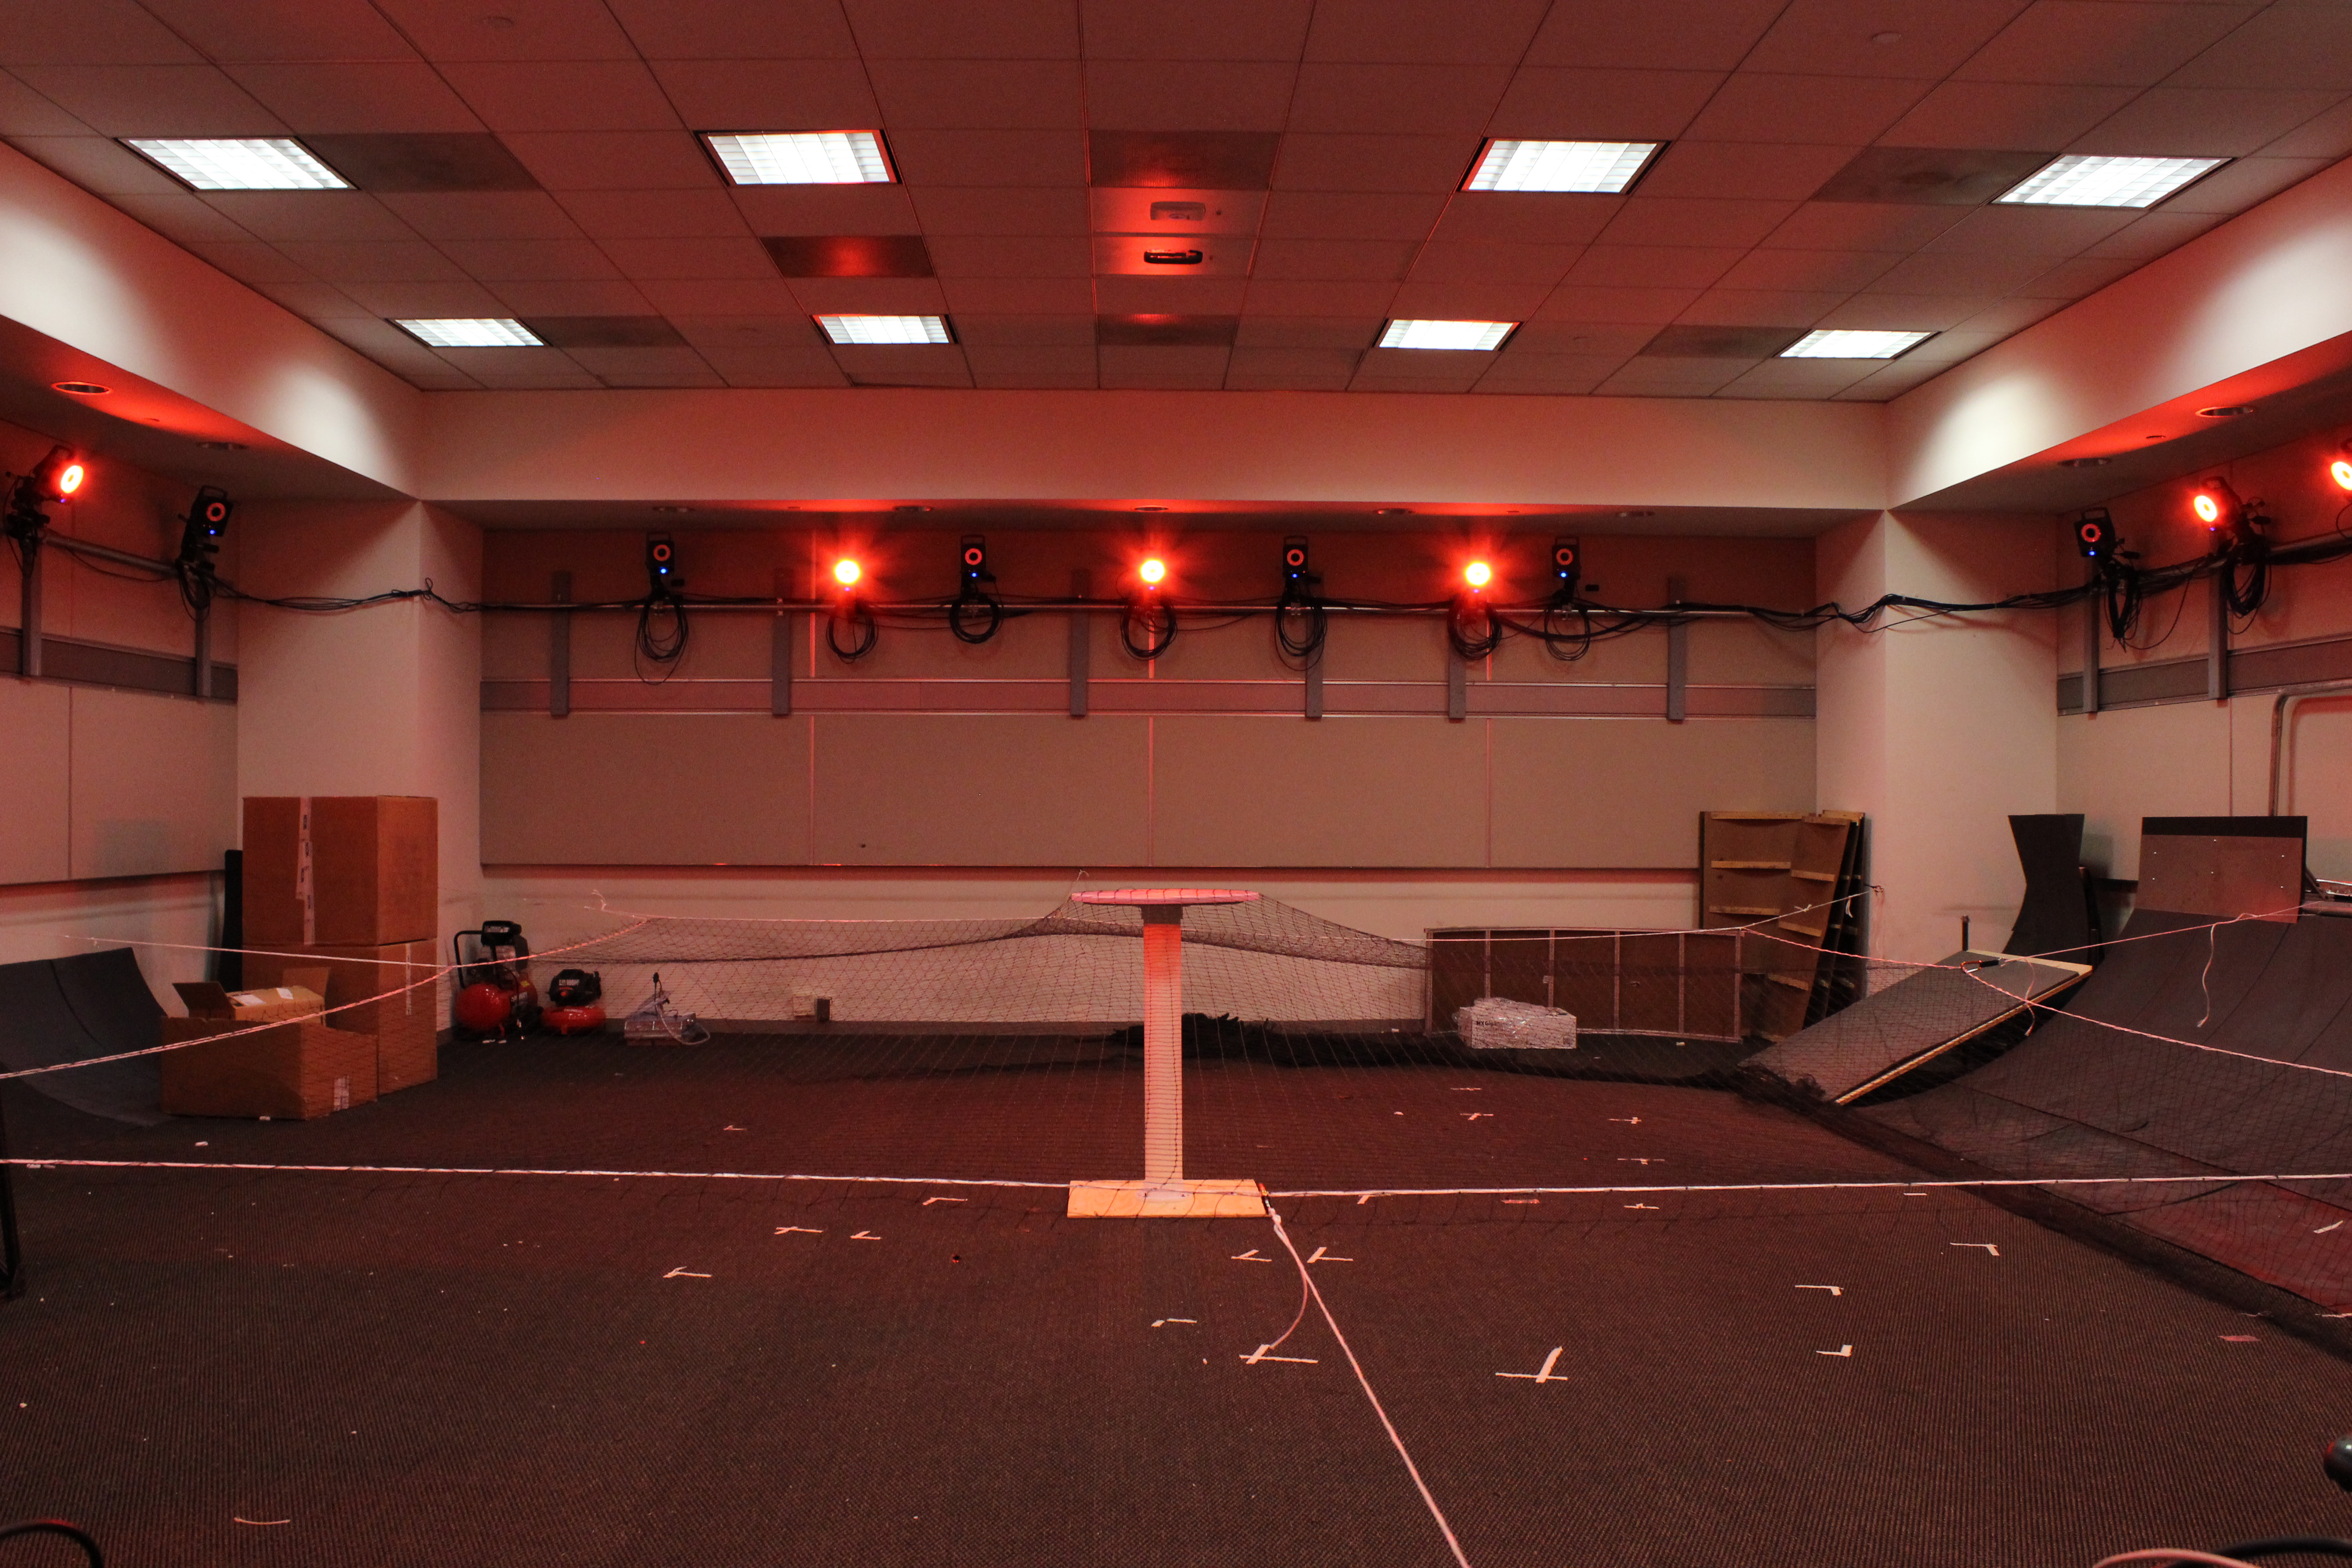
\includegraphics[width=0.45\columnwidth]{MoCa}}
	}
\centerline{
	\subfigure[\; Component test]{
		\includegraphics[width=0.45\columnwidth]{Spinning}}
		\hfill
	\subfigure[\; UAV on test rig]{
		\includegraphics[width=0.45\columnwidth]{UAV_OnTestStand.jpg}}
}	
\caption{The hardware is completed for the hexrotor UAV, and each component is tested at the Motion Capture Analysis (MoCa) laboratory of the George Washington University.}
\label{fig:hexrotorPicture}
\end{figure}

As preliminary tests, we controlled the hexrotor attitude about the $\vec b_3$ axis (yaw). A continuous desired command containing linear and nonlinear functions is applied to the controller. This command and the controlled system measurements are plotted in Figure \ref{fig:AttitudeControl}. This experiment shows that the applied control system is able to follow these tracking commands with moderate accuracy.

\begin{figure}
\centerline{
	\includegraphics[width=1.0\columnwidth]{Yaw_Test.png}}
\caption{The hexrotor UAV is fixed to a test rig such that yaw is controlled. The desired tracking command includes linear functions as well as half of a sinusoidal function.}
\label{fig:AttitudeControl}
\end{figure}


\section{Conclusions and Future Work}

This paper is focused on the design and development of a fully-actuated free-floating UAV for experimentation of geometric control of spacecraft maneuvers. Local coordinates such as Euler angles and quaternions are completely avoided in the controller design. Experimental results showed that variable pitch propeller actuators are capable of providing enough thrust in two directions such that hover may be achieved outside of a single plane of attitude. Numerical simulations serve to incorporate tested propeller ranges for a trajectory for which a quadrotor would not be capable. Preliminary results show that attitude control is possible and serve to show the system is operational in real time. Furthermore, the experimentation highlights the difficulties with variable pitch propeller actuation.

Future work involves further validation of the system and designing safe flight testing scenarios. With attitude control validated, only position control requires validation to test a free-floating hovering command. More complex attitude commands may be executed inside the admissible regions of hover so that the system may serve as an experimental testbed for complex rotational maneuvers.
%The next step is to perform experimental validation of the whole system. Some issues involving the communications lines between the COM and the IMU sensor made obtaining experimental results by the time of this paper submission difficult. We expect to obtain test results in the coming weeks.

\appendix{}

\subsection{Proof for Proposition 2}		

Substituting \refeqn{F} into \refeqn{vdot}, we have
\begin{align}
m\dot e_v & = mg e_3 + RF +\Delta_x  - m\ddot x \nonumber\\
& =-k_x e_x -k_v e_v -k_i e_i +\Delta_x. \label{eqn:evdot}
\end{align}
Therefore, $(e_x,e_v)=(0,0)$ with $e_i = \frac{\Delta_x}{k_i}$ is an equilibrium of the translational dynamics. Similarly, substituting \refeqn{M} into \refeqn{Wdot} and rearranging, we obtain
\begin{align}
J\dot e_\Omega = d\times e_\Omega - k_R e_R -k_\Omega e_\Omega -k_I e_I + \Delta_R,\label{eqn:JeWdot}
\end{align}
where $d=Je_\Omega + (2J-{\mathrm{tr}}J I) \Omega_d\in{\Re}^3$. Thus, $(e_R,e_\Omega)=(0,0)$ with $e_I=\frac{\Delta_R}{k_I}$ is an equilibrium of the rotational dynamics. However, the fact that $e_R=0$ does not imply that $R=R_d$. From the property (iii) of Proposition \ref{prop:1}, there are three additional attitudes satisfying $e_R=0$. This shows (i).

Next, let a Lyapunov function be
\begin{align}
{\mathcal{V}} = {\mathcal{V}}_1 + {\mathcal{V}}_2,
\end{align}
where ${\mathcal{V}}_1,{\mathcal{V}}_2$ are Lyapunov functions for the translational dynamics and the rotational dynamics, respectively defined as
\begin{align*}
{\mathcal{V}}_1 & = \frac{1}{2} m\|e_v\|^2 + c_1 e_x\cdot me_v + \frac{k_x}{2}\|e_x\|^2 + \frac{k_i}{2}\|e_i-\frac{\Delta_x}{k_i}\|^2,\\
{\mathcal{V}}_2 & = \frac{1}{2} e_\Omega\cdot Je_\Omega + c_2 e_R\cdot Je_\Omega + k_R \Psi + \frac{k_I}{2}\|e_I-\frac{\Delta_R}{k_I}\|^2.
\end{align*}
Using the results of Proposition \ref{prop:1}, we can show that
\begin{gather}
z_1^T M_{11} z_1 \leq {\mathcal{V}}_1-\frac{k_i}{2}\|e_i-\frac{\Delta_x}{k_i}\|^2 \leq z_1^T M_{12} z_1,\\
z_2^T M_{21} z_2 \leq {\mathcal{V}}_2-\frac{k_I}{2}\|e_I-\frac{\Delta_R}{k_I}\|^2 \leq z_2^T M_{22} z_2,\label{eqn:V2B}
\end{gather}
where $z_1=[\|e_x\|,\|e_v\|]^T$, $z_2=[\|e_R\|,\|e_\Omega\|]^T\in{\Re}^2$, and the matrices $M_{ij}\in{\Re}^{2\times 2}$ are defined as
\begin{gather*}
M_{11}=\frac{1}{2}\begin{bmatrix} k_x & -c_1m\\-c_1m & m\end{bmatrix},\quad
M_{12}=\frac{1}{2}\begin{bmatrix} k_x & c_1m\\c_1m & m\end{bmatrix},\\
M_{21}=\frac{1}{2}\begin{bmatrix} 2b_1k_R & -c_2\lambda_M\\-c_2\lambda_M & \lambda_m\end{bmatrix},\quad
M_{22}=\frac{1}{2}\begin{bmatrix} 2b_2k_R & c_2\lambda_M\\c_2\lambda_M & \lambda_M\end{bmatrix},
\end{gather*}
and $\lambda_m$ and $\lambda_M$ denote the minimum eigenvalue and the maximum eigenvalue $J$, respectively. Note that the upper bound of \refeqn{V2B} is satisfied in the following region of $\SO$:
\begin{align}
D=\{R\in{\SO}\,|\, \Psi < \psi <h_1\},\label{eqn:D}
\end{align}
for a positive constant $\psi$ from Proposition \ref{prop:1}.(v).

From \refeqn{ei}, \refeqn{evdot}, the time-derivative of ${\mathcal{V}}_1$ is given by
\begin{align*}
\dot{\mathcal{V}}_1 & = (e_v+c_1e_x)\cdot (-k_xe_x -k_ve_v-k_ie_i+\Delta_x) \\
&\quad + c_1m \|e_v\|^2 + k_x e_x\cdot e_v +k_i(e_i-\frac{\Delta_x}{k_i})\cdot(c_1e_x+e_v)\\
& = -c_1k_x\|e_x\|^2 -(k_v-c_1m)\|e_v\|^2 -c_1 k_v e_x\cdot e_v. 
\end{align*}
Its upper bound can be written as
\begin{align}
\dot{\mathcal{V}}_1 \leq -z_1^T W_1 z_1, 
\end{align}
where the matrix $W_1\in{\Re}^{2\times 2}$ is given by
\begin{align}
W_1 = \begin{bmatrix} c_1k_x & -\frac{1}{2}c_1 k_v \\
-\frac{1}{2}c_1 k_v & k_v-c_1m
\end{bmatrix}.\label{eqn:W1}
\end{align}

Next, from \refeqn{eI}, \refeqn{JeWdot}, the time-derivative of ${\mathcal{V}}_2$ is given by
\begin{align*}
\dot{\mathcal{V}}_2 & = (e_\Omega+c_2e_R)\cdot (d\times e_\Omega - k_R e_R -k_\Omega e_\Omega -k_I e_I +\Delta_R)\\
&\quad  + c_2\dot e_R \cdot Je_\Omega + k_Re_R\cdot e_\Omega +(k_Ie_I-\Delta_R)\cdot(c_2e_R+e_\Omega)\\
& = -c_2k_R \|e_R\|^2 -k_\Omega \|e_\Omega\|^2 +c_2\dot e_R\cdot Je_\Omega\\
&\quad + c_2 e_R\cdot (\hat d e_\Omega- k_\Omega e_\Omega).
\end{align*}
As the desired angular velocity is bounded from the assumption, there exists a constant $B>0$ satisfying
\begin{align*}
\|d\|=\|(2J-{\mathrm{tr}}[J]I)\Omega_d\| \leq  
B.
\end{align*}
And, since $\|\dot e_R\|\leq \frac{1}{\sqrt{2}}{\mathrm{tr}}[G]\|e_\Omega\|$ from Proposition \ref{prop:1},(vi), we can show that
\begin{align}
\dot{\mathcal{V}}_2 \leq -z_2^T W_2 z_2,\label{eqn:dotV2}
\end{align}
where $W_2\in{\Re}^{2\times 2}$ is defined as
\begin{align}
W_2 = \begin{bmatrix}
c_2 k_R & -\frac{c_2}{2}(k_\Omega+B_2)\\
-\frac{c_2}{2}(k_\Omega+B_2) & k_\Omega - \frac{c_2}{\sqrt{2}}{\mathrm{tr}}[G] \lambda_M
\end{bmatrix}.\label{eqn:W2}
\end{align}
In short, we have
\begin{align}
\dot{\mathcal{V}} \leq -z_1^T W_1 z_1-z_2^T W_2 z_2.
\end{align}
If the constants $c_1$ and $c_2$ are sufficiently small, we can show that all of the matrices $M_{ij},W_i$ for $i,j\in\{1,2\}$ are positive-definite. This implies that the zero equilibrium of the tracking errors, namely $(e_x,e_v,e_i,e_R,e_\Omega,e_I)=(0,0,\frac{\Delta_x}{k_i},0,0,\frac{\Delta_R}{k_I})$ is stable in the sense of Lyapunov, and $e_x,e_v,e_R,e_\Omega\rightarrow 0$ as $t\rightarrow 0$. 

But, the fact that $e_R\rightarrow 0$ does not necessarily imply $R\rightarrow R_d$, as $e_R=0$ at any one of four critical points of $\Psi$ from Proposition \ref{prop:1}.(iii): it is possible that the attitude converges to one of three undesired equilibria. Instead, we show instability of undesired equilibria to assure that the probability of converging to an undesired equilibrium is zero as follows.  At the first undesired equilibrium given by $R=R_d\exp \pi \hat e_1$, we have $\Psi=g_2+g_3$. Define ${\mathcal{W}}_2=(g_2+g_3)k_R-{\mathcal{V}}_2$. Then ${\mathcal{W}}_2=0$ at the first undesired equilibrium. Since
\begin{align*}
{\mathcal{W}}_2 &\geq -\frac{\lambda_M}{2}\|e_\Omega\|^2 +k_R(g_2+g_3-\Psi) -c_2\lambda_M\|e_R\|\|e_\Omega\| \\
&\quad -\frac{k_I}{2}\|e_I-\frac{\Delta_R}{k_I}\|^2.
\end{align*}
Due to the continuity of $\Psi$, at any arbitrary small neighborhood of the undesired equilibrium attitude, we can choose $R$ such that $g_2+g_3-\Psi>0$. Therefore, if $\|e_\Omega\|$ and $\|e_I-\frac{\delta_R}{k_I}\|$ are sufficiently small, then ${\mathcal{W}}_2>0$ at such attitudes. In short, at any arbitrary small neighborhood of the undesired equilibrium, there exists a domain where ${\mathcal{W}}_2>0$, and $\dot{\mathcal{W}}_2=-\dot{\mathcal{V}}_2>0$ in that domain from \refeqn{dotV2}. According to Theorem 4.3 at~\cite{Kha02}, the first undesired equilibrium is unstable. Instability of other two undesired equilibria can be shown similarly.

The region of attraction to the desired equilibrium excludes the stable manifolds to the undesired equilibria. But the dimension of the union of the stable manifolds to the unstable equilibria is less than the tangent bundle of $\SE$. Therefore, the measure of the stable manifolds to the unstable equilibrium is zero. Then, the desired equilibrium is referred to as \textit{almost} globally asymptotically stable with respect to $e_x,e_v,e_R$ and $e_\Omega$.

If this Lyapunov analysis is restricted to the domain $D$ given at \refeqn{D}, then the upper-bound of \refeqn{V2B} is also satisfied, and if the constant $c_2$ is chosen sufficiently small, the matrix $M_{22}$ is positive definite, i.e., the Lyapunov function is decrescent. These yield local exponential stability with respect to $e_x,e_v,e_R$ and $e_\Omega$. These show (ii) and (iii).

	
\acknowledgments

This research has been supported in part by NSF under the grants CMMI-1243000 (transferred from 1029551), CMMI-1335008, and CNS-1337722.

		
		
\bibliography{BibMaster}
\bibliographystyle{IEEEtran}

\thebiography

\begin{biographywithpic}
{Evan Kaufman}{EvanKaufman.eps}
received his B.S. in Mechanical Engineering from Bucknell University in 2012. He is currently pursuing a Ph.D. in Aerospace Engineering at The George Washington University. Evan's research interests include nonlinear control, rigid body dynamics, and optimal estimation. He is currently focused on applications of geometric nonlinear control.
\end{biographywithpic}

\begin{biographywithpic}
{Kiren Caldwell}{KirenCaldwell.eps}
is a senior at The George Washington University majoring in Mechanical Engineering with a concentration in aerospace engineering. He is interested in applications of controls for UAVs and other aeronautical vehicles.
\end{biographywithpic}

\vspace{20pt}

\begin{biographywithpic}
{Daewon Lee}{DaewonLee.eps}
received the B.S. and Ph.D. in Mechanical and Aerospace Engineering from Seoul National University (SNU), Seoul, Korea, in 2005 and 2012, respectively. Currently, he is a postdoc researcher at The George Washington University. His research interests include applications of nonlinear control, vision-based control of UAVs and aerial manipulation of UAVs.
\end{biographywithpic}

\begin{biographywithpic}
{Taeyoung Lee}{TaeyoungLee.eps}
is an assistant professor at the Department of Mechanical and Aerospace Engineering of the George Washington University. He received his doctoral degree in
Aerospace Engineering, and his master's degree in Mathematics at the University of Michigan in 2008. His research interests include geometric mechanics, geometric nonlinear control, optimization, estimation, and computational mechanics with applications to complex aerospace systems.
\end{biographywithpic}

		
%\subsection{Biography}
%
%
%\begin{wrapfigure}{l}{0.15\textwidth}
%\vspace{-20pt}
%  \begin{center}
%    \includegraphics[]{EvanKaufman}
%  \end{center}
%%\vspace{-20pt}
%  \begin{center}
%    \includegraphics[]{KirenCaldwell}
%  \end{center}
%%\vspace{-20pt}
%  \begin{center}
%    \includegraphics[]{DaewonLee}
%  \end{center}
%%\vspace{-20pt}
%  \begin{center}
%    \includegraphics[]{TaeyoungLee}
%  \end{center}
%%\vspace{-20pt}
%\end{wrapfigure}
%
%\vspace{30pt}
%\emph{{\bf Evan Kaufman} received his B.S. in Mechanical Engineering from Bucknell University in 2012. He is currently pursuing a Ph.D. in Aerospace Engineering at The George Washington University. Evan's research interests include nonlinear control, rigid body dynamics, and optimal estimation. He is currently focused on applications of geometric nonlinear control.}
%
%\vspace{20pt}
%Kiren Caldwell is a senior at The George Washington University majoring in Mechanical Engineering with a concentration in aerospace engineering. He is interested in applications of controls for UAVs and other aeronautical vehicles.
%
%\vspace{30pt}
%Daewon Lee received the B.S. and Ph.D. in Mechanical and Aerospace Engineering from Seoul National University (SNU), Seoul, Korea, in 2005 and 2012, respectively. Currently, he is a postdoc researcher at The George Washington University. His research interests include applications of nonlinear control, vision-based control of UAVs and aerial manipulation of UAVs.
%
%\vspace{5pt}
%Taeyoung Lee is an assistant professor at the Department of Mechanical and Aerospace Engineering of the George Washington University. He received his doctoral degree in
%Aerospace Engineering, and his master's degree in Mathematics at the University of Michigan in 2008. His research interests include geometric mechanics, geometric nonlinear control, optimization, estimation, and computational mechanics with applications to complex aerospace systems.
%

\end{document}



%%%%%%%%%%%%%%%%%%%%%%%%%%%%%%%%%%%%%%
\section{Introduction}
%%%%%%%%%%%%%%%%%%%%%%%%%%%%%%%%%%%%%%
The annual IEEE Aerospace Conference is a venue for engineers and scientists to present their work to one another. Please submit a paper only if you or a coauthor are committed to attend and present it personally.

An IEEE Aerospace Conference paper is comprised of standard parts described in Section 2 of this paper. Section 3 briefly describes the manuscript style and Section 4 the submission deadlines and procedures. Section 5 discusses presentation of papers at the conference. The Best Paper Award and paper publication are described in Section 6. Section 7 provides a summary.

Proper formatting of your paper as specified in this document contributes to the successful production of these documents. All papers are also published in PDF format on the IEEE Xplore Web based system, shortly after the conference concludes.

A double-column format is required, although figures, tables, and equations may be full-page width. Specifications are listed for typeface, type size, headings, column separation, margins, and other style parameters.

Where this document is silent on a formatting question, it is because it is not important or is the writer�s option. When in doubt make a choice that makes your document most readable. English is the official language of the conference, and the official page size is 8.5 x 11 inches�--do not use A4 paper size.



%%%%%%%%%%%%%%%%%%%%%%%%%%%%%%%%%%%%%%%%%%%
\section{Paper Organization}
%%%%%%%%%%%%%%%%%%%%%%%%%%%%%%%%%%%%%%%%%%%
IEEE papers consist of a minimum of nine parts.

\subsection{Title}
The title should indicate the subject of the paper as briefly as possible. The maximum length, including spaces, is 100 characters.

\subsection{Author(s)}
Names of all authors, their affiliations, postal addresses, phone numbers, and e-mail addresses should follow the title, centered on the full width of the page. Do not include titles or degrees except for military rank. Multiple authors may be listed two or three across and as deep as needed. Large numbers of authors should be grouped by address.

\subsection{Abstract}
An abstract of about 150 words should concisely describe the work being reported, its methodology, principal results and significance.

\subsection{Table of Contents}
Major headings and their page numbers are listed in the Table of Contents.

\subsection{Introduction}
The introduction provides background information, such as previous work, and describes how the paper is organized.

\subsection{Body}
The body describes the work in detail and discusses its application. The body should be organized into logical sections with headings and subheadings and be illustrated with figures and tables. Subsidiary information can be relegated to footnotes.

\subsection{Conclusions}
Conclusions should clearly state principal results of the work, its significance, limitations, advantages, and applications. Recommendations for further work are also encouraged.

\subsection{References}
List and number all bibliographical references at the end of the paper.

\subsection{Biography}
Provide a short biography for each author, which can include title, fields of expertise, work experience, education, and relevant personal information. Also include a 1.25 inch wide x 1.5 inch high headshot (at 300 dpi) of each author.

\subsection{Additions}
Add appendices and acknowledgments, if appropriate.



%%%%%%%%%%%%%%%%%%%%%%%%%%%%%%%%%%%%%%%%%%%%%
\section{Manuscript Style}
%%%%%%%%%%%%%%%%%%%%%%%%%%%%%%%%%%%%%%%%%%%%%

\subsection{Paper Length}
The paper may be 6 to 20 pages in length.

\subsection{Copyright Notice}
A copyright notice must be placed as a footnote on the first page of the paper. Do not number this footnote. Choose an appropriate alternative from the list of three below:
\begin{itemize}
  \item [(1)] For papers in which all authors are employed by the US government, the notice is: \\{\bf U.S. Government work not protected by U.S. copyright} \\
  \item [(2)] For papers in which all authors are employees of a Crown Government (UK, Canada, Australia), the notice is: \\{\bf 978-1-4799-1622-1/14/\$31.00 \copyright2014 Crown} \\
  \item [(3)] For all other papers the notice is: \\{\bf 978-1-4799-1622-1/14/\$31.00 \copyright2014 IEEE}
\end{itemize}

\subsection{Paper, Margins, and Spacing}
Format your electronic submission to 8.5 x 11 inch page size in double-column format with 0.75 inch margins on each side, top and bottom. There should be 0.25 inch between columns, which are justified both right and left.

Lines of text should be single-spaced, except for double spacing before headings and space-and-a-half after.

\subsection{Headers and Footers}
No headers are permitted. Utilize footers only for page numbers, which are centered at the bottom of each page.

\subsection{Headings}
\subsubsection{Major Headings}
Centered in the column with a double space before and space-and-a-half after.
\subsubsection{Subheadings}
Italicized and placed flush on the left-hand margin on a separate line. Use a double space before and space-and-a-half after.
\subsubsection{Subsubheadings}
Italicized, followed by an em dash and run in at the beginning of the paragraph. This paragraph has a correctly formatted subsubheading.

\subsection{Other Elements}
\subsubsection{Equations}
Equations should be centered in the column. When numbering an equation, enclose the number in parentheses placed flush with the right-hand margin of the column, as shown in the sample equations that follow.
\begin{equation}
{\bf F}=m{\bf a}
\end{equation}
\begin{equation}
e=mc^2
\end{equation}

Mathematical derivations and proofs should be developed in appendices.

\subsubsection{Figures}
Place figures as close to the text reference as possible. Center figure titles directly below the figure, as shown in Figure 1.

Figures should be sized for easy reading. No lettering in a figure should be smaller than 10 points. Scan photographs at a 300-dpi resolution and embed them in the paper. High-resolution images should be reduced to 300 dpi at the size they will be printed.

\begin{figure*}
\centering
\includegraphics[width=4in]{Placeholder.eps}
\caption{Here is an example of a figure that spans both columns.}
\label{FlowChart}
\end{figure*}

\subsubsection{Tables}
Place tables as close to the text reference as possible. Use the full width of the page for legibility, if required. Center table titles directly {\bf above} the table.

\subsubsection{Footnotes}
All footnotes\footnote{This is an example of a footnote.} following the IEEE copyright notice are numbered consecutively. 

%%%%%%%%%%%%%%%%%%%%%%%%%%%%%%%%%%%%%%%%%%%%%%%%%%%%%
\section{Paper Submission}
Submission due dates and deadlines are given in Table \ref{DueDates}.

\begin{table}
\renewcommand{\arraystretch}{1.3}
\caption{\bf Summary of Due Dates}
\label{DueDates}
\centering
\begin{tabular}{|c|c|}
\hline
\bfseries Event & \bfseries Due Date \\
\hline\hline
Abstracts Due               & July 15, 2013 \\
Review Paper {\bf Deadline} & October 25, 2013 \\
Revised papers Due          & January 5, 2014\\
IEEE Copyright Form Due     & January 5, 2014 \\
\hline
\end{tabular}
\end{table}

\subsection{Abstract}
An abstract of about 600 words describing the planned content of the paper must be submitted electronically at the conference website.

\subsection{Review Paper}
The paper submitted for review must be a complete, fully formatted, and proofread manuscript, ready for publication. NO paper submitted for review after the deadline will be reviewed or admitted to the conference.

\subsection{Final Paper}
Following receipt of review comments, make appropriate revisions to the paper and submit a final version for publication.

\subsection{IEEE copyright Form}
An IEEE Copyright Release Form for each paper, signed by the author or author�s employer, is due with the final paper. Copyright forms are available at the conference website and can be submitted electronically at the IEEE site linked for this purpose.

\subsection{ITAR Compliance}
International Traffic in Arms Regulation (ITAR) controls the export and import of defense articles and defense services as detailed in the U.S. Munitions List \cite{ITAR}.

Authors who are U.S. nationals (including green card holders), work for a U.S.-based organization regardless of where they are physically located, or work at a U.S. location of a non-U.S.-based organization, must ensure that ITAR compliance has been obtained for any and all papers submitted to IEEE for publication.

\subsection{Organizational Approval}
Authors are expected to obtain any needed clearances for their work to be freely published by the IEEE. Submission of your paper implies that it has received the proper clearances from your company, affiliation, or organization.

\subsection{Electronic Submission}
Before Submitting your abstract or paper:
\begin{itemize}
  \item [1)] Scan your document with a current anti-virus product. (If a virus is detected, your file willl be deleted) \\
  \item [2)] Remove passwords or other protection from your file that would prevent it from being opened. \\
  \item [3)] Submit a PDF version of your abstract of paper via the website.
\end{itemize}

%%%%%%%%%%%%%%%%%%%%%%%%%%%%%%%%%%%%%%%%%%%%%%%%%%%%%
\section{Presentation at the Conference}
%%%%%%%%%%%%%%%%%%%%%%%%%%%%%%%%%%%%%%%%%%%%%%%%%%%%%
Prepare a presentation to be delivered at the conference, using Microsoft PowerPoint or similar software, that summarizes the major concepts of your paper.

\subsection{Allotted Time}
Time allotted for presentations is 18 minutes, with an additional 5 minutes for questions. The time limit will be strictly enforced.

\subsection{Projection}
A projector and screen will be set up in each meeting room. Bring your slide set on a laptop to plug in to the projector. Also bring a copy of your presentation on a USB drive, in case your session chair chooses to consolidate all the presentations on a single laptop before the session starts.

\subsection{Presentation}
Tips on giving the presentation will be sent to registered authors in advance of the conference.


\subsection{Pre-Recorded Presentation Alternative}
For authors who prefer to pre-record a narration of their slides (for example, by using the Record Narration feature of Microsoft PowerPoint), the conference will set up an Electronic Presentation Hall (EPH). EPH presentations run autonomously during specific times at the conference. The author must be registered for at least one day of the conference and may stand by during one or more of the view times to answer viewer questions.

\subsection{Special Displays}
Displays of hardware or software an author believes to be of wide interest to conference attendees may be set up with permission of the Technical Program Committee and by special arrangement with the Conference Manager.

%%%%%%%%%%%%%%%%%%%%%%%%%%%%%%%%%%%%%%%%%%%%%%%%%%%%%
\section{Best Paper Award and Publication}
%%%%%%%%%%%%%%%%%%%%%%%%%%%%%%%%%%%%%%%%%%%%%%%%%%%%%
\subsection{Best Paper Award}
A Best Paper Award is given each year for excellence in technical innovation and exposition in the written paper. The selection is conducted prior to the conference and the award is presented at the Conference.

\subsection{Publication}
Papers presented at the IEEE AEROSPACE Conference are published in two forms:
\begin{itemize}
  \item [1)] On a CD-ROM distributed to registrants at the conference \\
  \item [2)] In the official Conference Proceedings on the web- based IEEE Xplore System following the conference
\end{itemize}


%%%%%%%%%%%%%%%%%%%%%%%%%%%%%%%%%%%%%%%%%%%%%%%%%%%%%
\section{Examples of Formatting} \label{s:examples}
%%%%%%%%%%%%%%%%%%%%%%%%%%%%%%%%%%%%%%%%%%%%%%%%%%%%%
Figure \ref{OneColumn} shows an example of a figure spanning a single column.

\begin{figure}
\centering
\includegraphics[width=3.25in]{Placeholder.eps}
\caption{A single column figure.}
\label{OneColumn}
\end{figure}


%%%%%%%%%%%%%%%%%%%%%%%%%%%%%%%%%%%%%%%%%%%%%%%%%%%%%
\section{Summary}
%%%%%%%%%%%%%%%%%%%%%%%%%%%%%%%%%%%%%%%%%%%%%%%%%%%%%
This Author�s Instructions document serves as a template for papers prepared for the 2014 IEEE Aerospace Conference. All paper submissions are accomplished online, through the IEEE Aerospace Conference website at www.aeroconf.org \cite{AeroConf}.





%%%%%%%%%%%%%%%%%%%%%%%%%%%%%%%%%%%%%%%%%%%%%%%%%%%%%%%%%%%%%%%%%%%%%%%%%%%%%%%%%%%%%%%%%%%%%%%%%
\appendices               % note there is no {} to put a title. Each appendix has its own title
%%%%%%%%%%%%%%%%%%%%%%%%%%%%%%%%%%%%%%%%%%%%%%%%%%%%%%%%%%%%%%%%%%%%%%%%%%%%%%%%%%%%%%%%%%%%%%%%%
% For a single appendix, use the \appendix{} keyword and do not use the \section command.

\section{More Information}        % first appendix
%%%%%%%%%%%%%%%%%%%%%%%%%%
This is the first appendix. 

\subsection{Comments}
If you have only one appendix, use the ``appendix'' keyword.

\subsection{More Comments}
Use section and subsection keywords as usual.

\section{Yet More Information}    % second appendix
%%%%%%%%%%%%%%%%%%%%%%%%%%%%%%
This is the second appendix.



%%%%%%%%%%%%%%%%%%%%%%%%%%%%%%%%%%%%%%%%%%%%%%%%%%%%%%%%%%%%%%%%%%%%%%%%%%%%%%%%%%%%%%%%%%%%%%%%%%%%%%
\acknowledgments
The authors thank the Office of Naval Research for funding this project.



%%%%%%%%%%%%%%%%%%%%%%%%%%%%%%%%%%%%%%%%%%%%%%%%%%%%%%%%%%%%%%%%%%%%%%%%%%%%%%%%%%%%%%%%%%%%%%%%%%%%%%
\bibliographystyle{IEEEtran}
%\bibliography{IEEEabr,MyBibFile}
\begin{thebibliography}{1}

\bibitem{ITAR}
U.S. Munitions List, Sections 38 and 47(7) of the Arms Export Control Act (22 U.S.C 2778 and 2794(7).

\bibitem{AeroConf}
Aerospace Conference Web site: www.aeroconf.org/

\end{thebibliography}


%%%%%%%%%%%%%%%%%%%%%%%%%%%%%%%%%%%%%%%%%%%%%%%%%%%%%%%%%%%%%%%%%%%%%%%%%%%%%%%%%%%%%%%%%%%%%%%%%%%%%%
\thebiography
%% This biostyle allows you to insert your photo size 1in X 1.25in
\begin{biographywithpic}
{Erica Deionno}{Deionno.eps}
received her B.S. and M.S. degrees in chemistry from UCLA in 1998 and a Ph.D. in chemistry in 2006. She is currently a member of the technical staff at The Aerospace Corporation. Her current research activities include radiation testing and modeling of emerging resistive RAM technologies and modeling space solar cell degradation.
\end{biographywithpic} 

\begin{biographywithpic}
{Jane Smith}{blankpic.eps}
received her B.S. degree in Electrical Engineering in 1985 and a Ph.D. in Aerospacel Engineering from the Massachusettes Institute of Technology in 1990. She is currently a professor of Aerospace Engineering at the University of Nowhere. Her interests include secure communications and space exploration.

\end{biographywithpic}

\bibliography{BibMaster}
\bibliographystyle{IEEEtran}



\end{document}

%\begin{itemize}
%\item Variable-pitch prop
%\begin{itemize}
%\item need to generate thrust along both directions
%\item configuration of variable pitch prop
%\begin{itemize}
%\item  description, BLDC motor and PWM servo, ESC and i2c conversion, CAD model and 3D printing of servo place holder
%\end{itemize}
%\end{itemize}
%\item  Motor calibration
%\begin{itemize}
%\item description, BLDC motor and PWM servo, ESC and i2c conversion, CAD model and 3D printing of servo place holder
%\end{itemize}
%\end{itemize}
